\documentclass[default]{beamer}
\setbeamertemplate{navigation symbols}{}

\usetheme{CambridgeUS}
%\useoutertheme{infolines}
\usecolortheme{beaver}

\usepackage[utf8]{inputenc}					% Выбор языка и кодировки
\usepackage[english]{babel}	% Языки: русский, английский
\usepackage{csquotes}

\usepackage{tikz}
\usetikzlibrary{arrows,shapes,calc}
\everymath{\displaystyle}
\tikzstyle{every picture}+=[remember picture]

\usepackage{animate}
\usepackage{fp}
\usepackage{textpos}

\usepackage[
	language=auto,
	autolang=other,
	backend=biber,
	style=authortitle,
	sorting=ydnt,
	maxbibnames=5
]{biblatex}
\addbibresource{panov_bica2017.bib}
				
\DeclareSourcemap{
	\maps[datatype=bibtex, overwrite]{
		\map{
			\step[fieldset=langid, fieldvalue=english]
			\step[fieldset=doi, null]
			\step[fieldset=issn, null]
			\step[fieldset=isbn, null]
			\step[fieldset=url, null]
			\step[fieldsource=language, fieldset=langid, origfieldval]
		}
	}
}
\DeclareBibliographyDriver{std}{%
	\usebibmacro{bibindex}%
	\usebibmacro{begentry}%
	\usebibmacro{author/editor+others/translator+others}%
	\setunit{\labelnamepunct}\newblock
	\usebibmacro{title}%
	\newunit\newblock
	\usebibmacro{maintitle+booktitle}
	\newunit\newblock
	\usebibmacro{journal}%
	\newunit\newblock
	\usebibmacro{date}%
	\newunit\newblock
	\usebibmacro{finentry}
}
\DeclareBibliographyAlias{article}{std}
\DeclareBibliographyAlias{book}{std}
\DeclareBibliographyAlias{inproceedings}{std}
\DeclareBibliographyAlias{incollection}{std}

\graphicspath{{../../images/}} 			% Пути к изображениям

\makeatletter
\setbeamertemplate{footline}
{
	\leavevmode%
	\hbox{%
		\begin{beamercolorbox}[wd=.333333\paperwidth,ht=2.25ex,dp=1ex,center]{author
				in head/foot}%
			\usebeamerfont{author in
				head/foot}\insertshortauthor~~\beamer@ifempty{\insertshortinstitute}{}{(\insertshortinstitute)}
		\end{beamercolorbox}%
		\begin{beamercolorbox}[wd=.333333\paperwidth,ht=2.25ex,dp=1ex,center]{title in
				head/foot}%
			\usebeamerfont{title in head/foot}\insertshorttitle
		\end{beamercolorbox}%
		\begin{beamercolorbox}[wd=.333333\paperwidth,ht=2.25ex,dp=1ex,right]{date in
				head/foot}%
			\usebeamerfont{date in head/foot}\insertshortdate{}\hspace*{1em}
			\insertframenumber{}\hspace*{2ex} 
		\end{beamercolorbox}
	}%
	\vskip0pt%
}

\addtobeamertemplate{frametitle}{}{
	\begin{textblock*}{100mm}(\textwidth-35pt,-20pt)
		
\includegraphics[width=1.5cm]{misc/logos/frccsc.png}
	\end{textblock*}
}

\newcommand{\predmatr}[3]{
	\node[ell, rectangle, minimum height = 15, minimum width = 7.5]  at (#1 pt,#2 pt) {}; 
	\node[ellf, rectangle, minimum height = 15, minimum width = 7.5] at (#1+7.5 pt,#2 pt) {};
	\node[minimum height = 15, minimum width = 15] (#3) at (#1+3.3pt,#2 pt) {};
	\draw[ell] (#1+7.5 pt,#2+7.5 pt) -- (#1 +7.5 pt,#2-7.5 pt);
}
\renewcommand*{\bibfont}{\tiny}
\setlength\bibitemsep{-5pt}

\begin{document}
	
	\title[PathPlan+RL]{Grid Path Planning with Deep Reinforcement Learning: Preliminary Results}
	\author[Panov, Suvorov, Yakovlev]{Alelsandr Panov, Roman Suvorov and Konstantin Yakovlev}
	\institute[RAS]{Federal Research Center ``Computer Science and Control''\\Russian Academy of Sciences (RAS)\\National Research University Higher School of Economics\\\textbf{Moscow}}
	\date[August 2 -- FIERCES 2017]{August 2 -- Fierces on BICA 2017} 
		
	\begin{frame}
		\titlepage
		\centering
		
\includegraphics[height=20pt]{misc/logos/ras_en.png} \hspace{10pt}
		
\includegraphics[height=20pt]{misc/logos/frccsc.png} \hspace{10pt}
		
\includegraphics[height=20pt]{misc/logos/hse.png}
	\end{frame}

	\section{Intro}
	\subsection{Sign based world model}

	\begin{frame}
		\frametitle{Sign based world model}
		\onslide<1->{
			{\footnotesize
				A component of knowledge representation is a sign:
				\begin{itemize}
					\item in sense of cultural-historical approach by L. Vygotsky,
					\item in sense of activity theory by A. Leontiev.
				\end{itemize}
			}
		}
		\onslide<2->{
			\begin{columns}
				\begin{column}{0.4\textwidth}
					\centering
					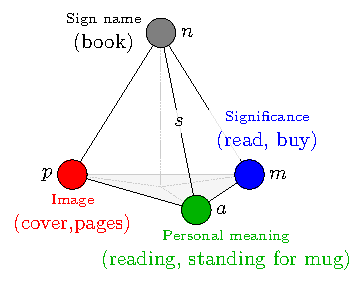
\includegraphics[width=0.7\textwidth]{signs/en/sign_colored_rita}
				\end{column}
				
			}
			\onslide<3->{
				\begin{column}{0.6\textwidth}
					\begin{columns}
						\begin{column}{0.5\textwidth}
							\centering
							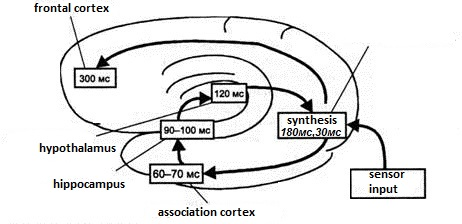
\includegraphics[width=\textwidth]{misc/phisio/ivan_cyrc_en}
						\end{column}
						\begin{column}{0.5\textwidth}
							\centering
							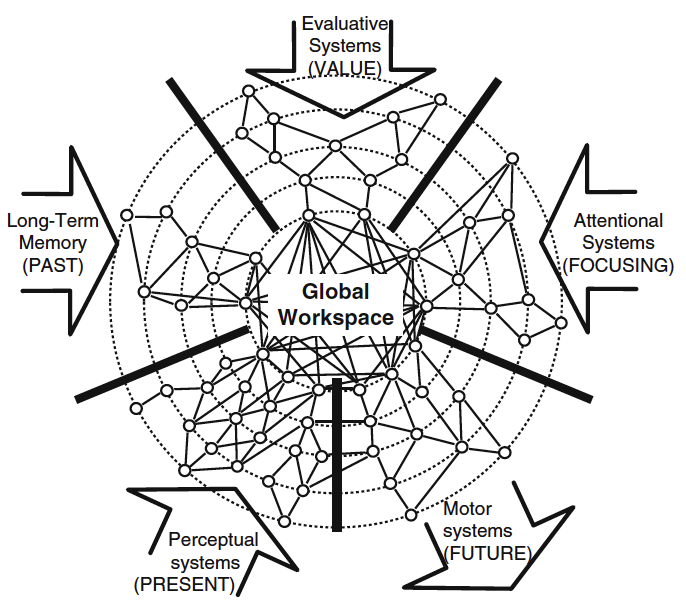
\includegraphics[width=\textwidth]{misc/phisio/workspace}
						\end{column}
					\end{columns}
				\end{column}
			\end{columns}
			
			
			{\footnotesize
				Supported ideas in psychology and biology:
				\begin{itemize}
					\item neurophysiological data (Edelman, Ivanitsky, Mountcastle etc.),
					\item two and three levels psychological theories (Stanovich, Kahneman).
				\end{itemize}
			}
			\vspace{-5pt}
			\nocite{*}
			\printbibliography[keyword={sign}, resetnumbers=true]
		}
	\end{frame}
				
	\begin{frame}
		\frametitle{Modelling of world model}
		\begin{columns}
			\begin{column}{0.5\textwidth}
				\centering
				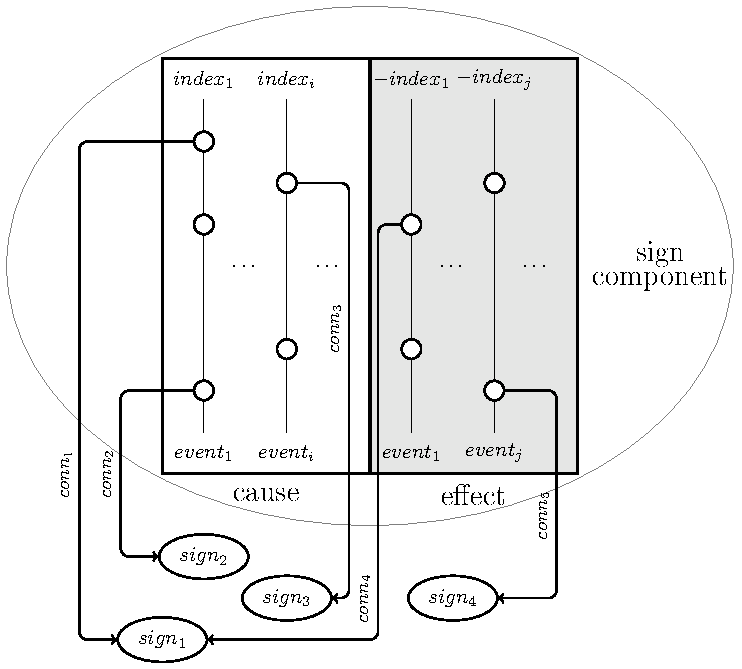
\includegraphics[width=0.7\textwidth]{causnet/caus_matr}
				
				
			\end{column}
			\begin{column}{0.5\textwidth}
				\centering
				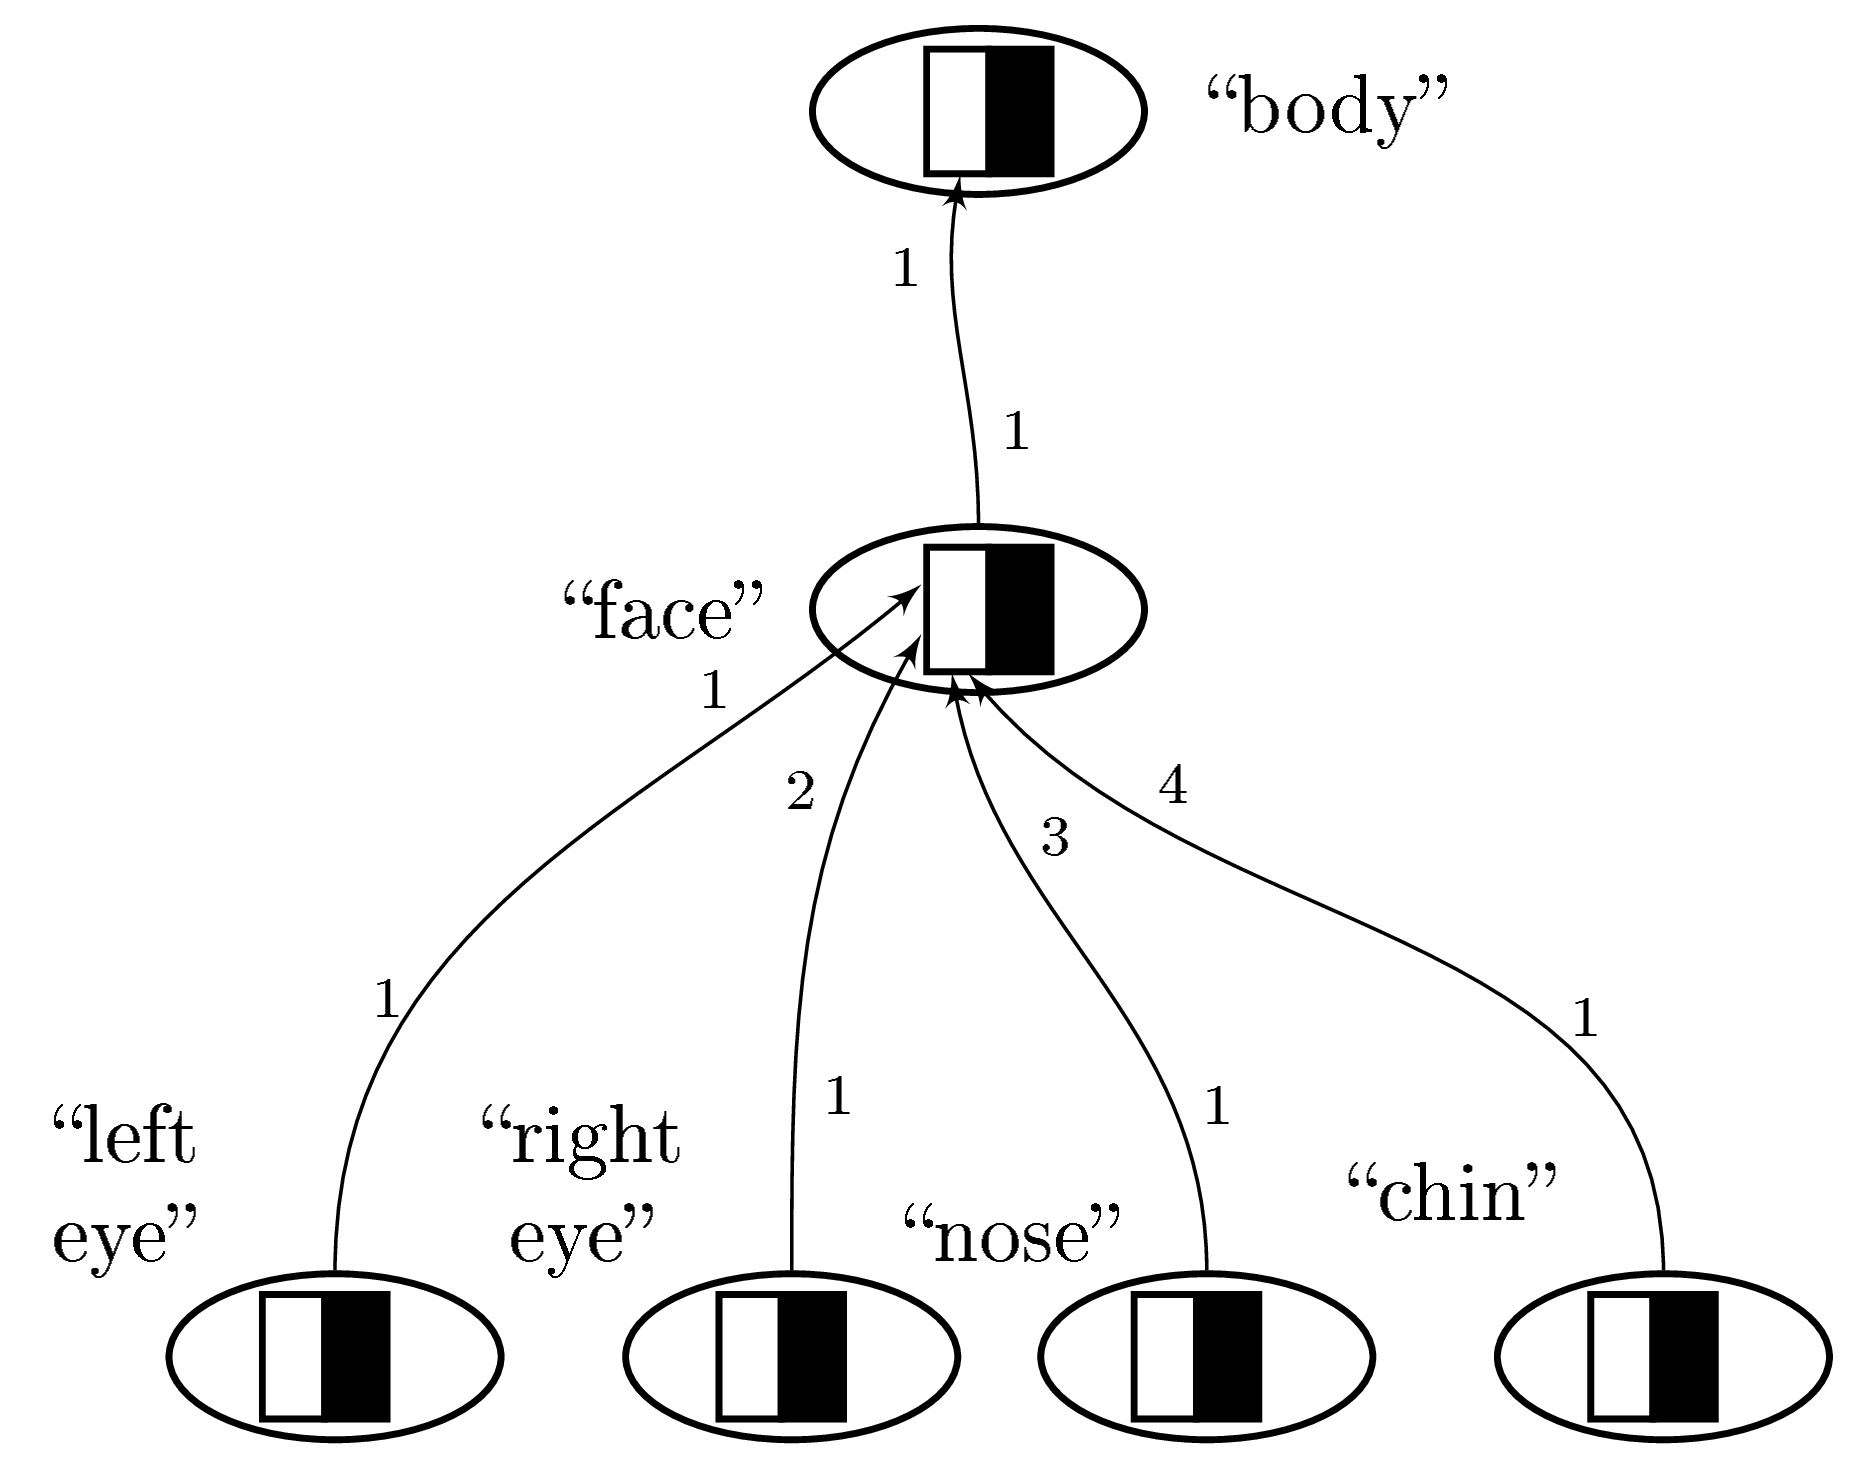
\includegraphics[page=1,width=0.7\textwidth]{examples/causnet/caus_net_en}
			\end{column}
		\end{columns}
		\begin{columns}
			\begin{column}{0.5\textwidth}
				\centering
				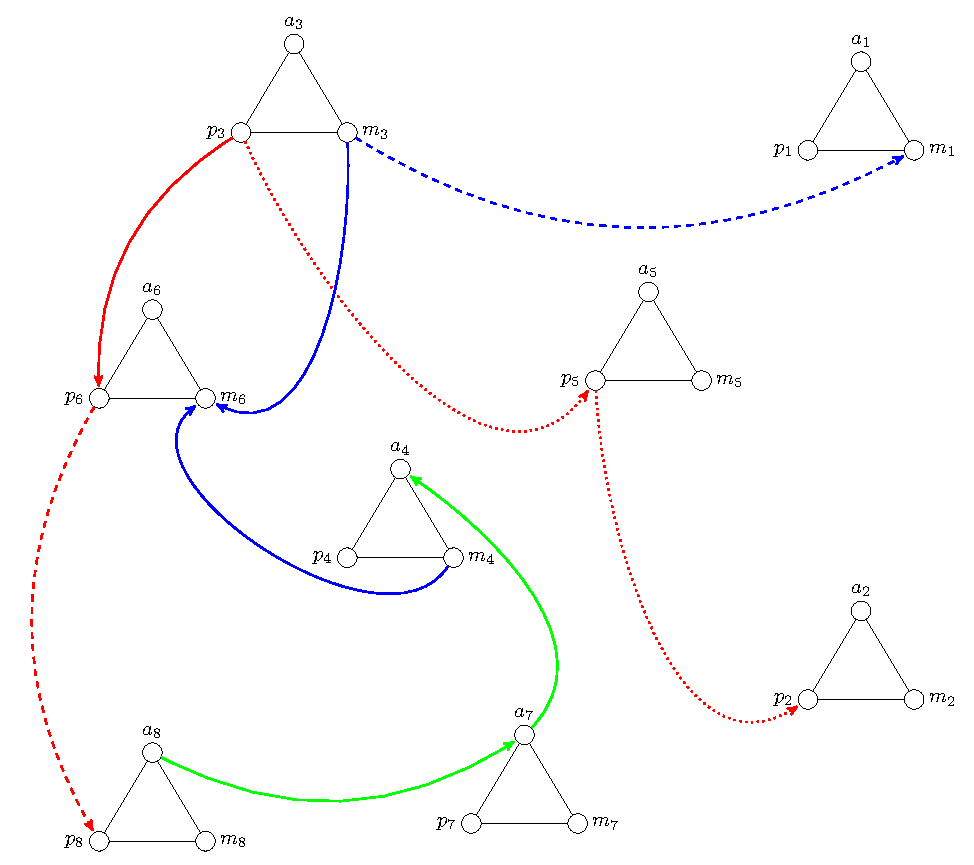
\includegraphics[width=0.7\textwidth]{signnet/signs_net}
			\end{column}
			\begin{column}{0.5\textwidth}
				Sign based world model (semiotic network):
				\[\Omega=\langle W_p, W_m, W_a, R_n, \Theta \rangle\]
				
				\vspace{-5pt}
				\nocite{*}
				\printbibliography[keyword={signmodel}, resetnumbers=true]
			\end{column}
		\end{columns}
	\end{frame}

	\subsection{Applications}
	
	\begin{frame}
		\frametitle{Applications}

		\footnotesize
		\begin{columns}
			\begin{column}{0.43\textwidth}
				\begin{itemize}
					\item Cognitive functions modeling and construction of models that explain psychological phenomena.
					\item Algorithm of synthesizing the plan of behavior (algorithms MAP, MultiMAP, GoalMAP).
					\item Solving symbol grounding and symbol anchoring problems.
					\item Reconstruction of sign based world model of the actor based on texts.
					\item Text generation based on specific world models (virtual assistants).
					\item Multi-level architectures of control (robotic systems).
				\end{itemize}
				
			\end{column}
			\begin{column}{0.57\textwidth}
				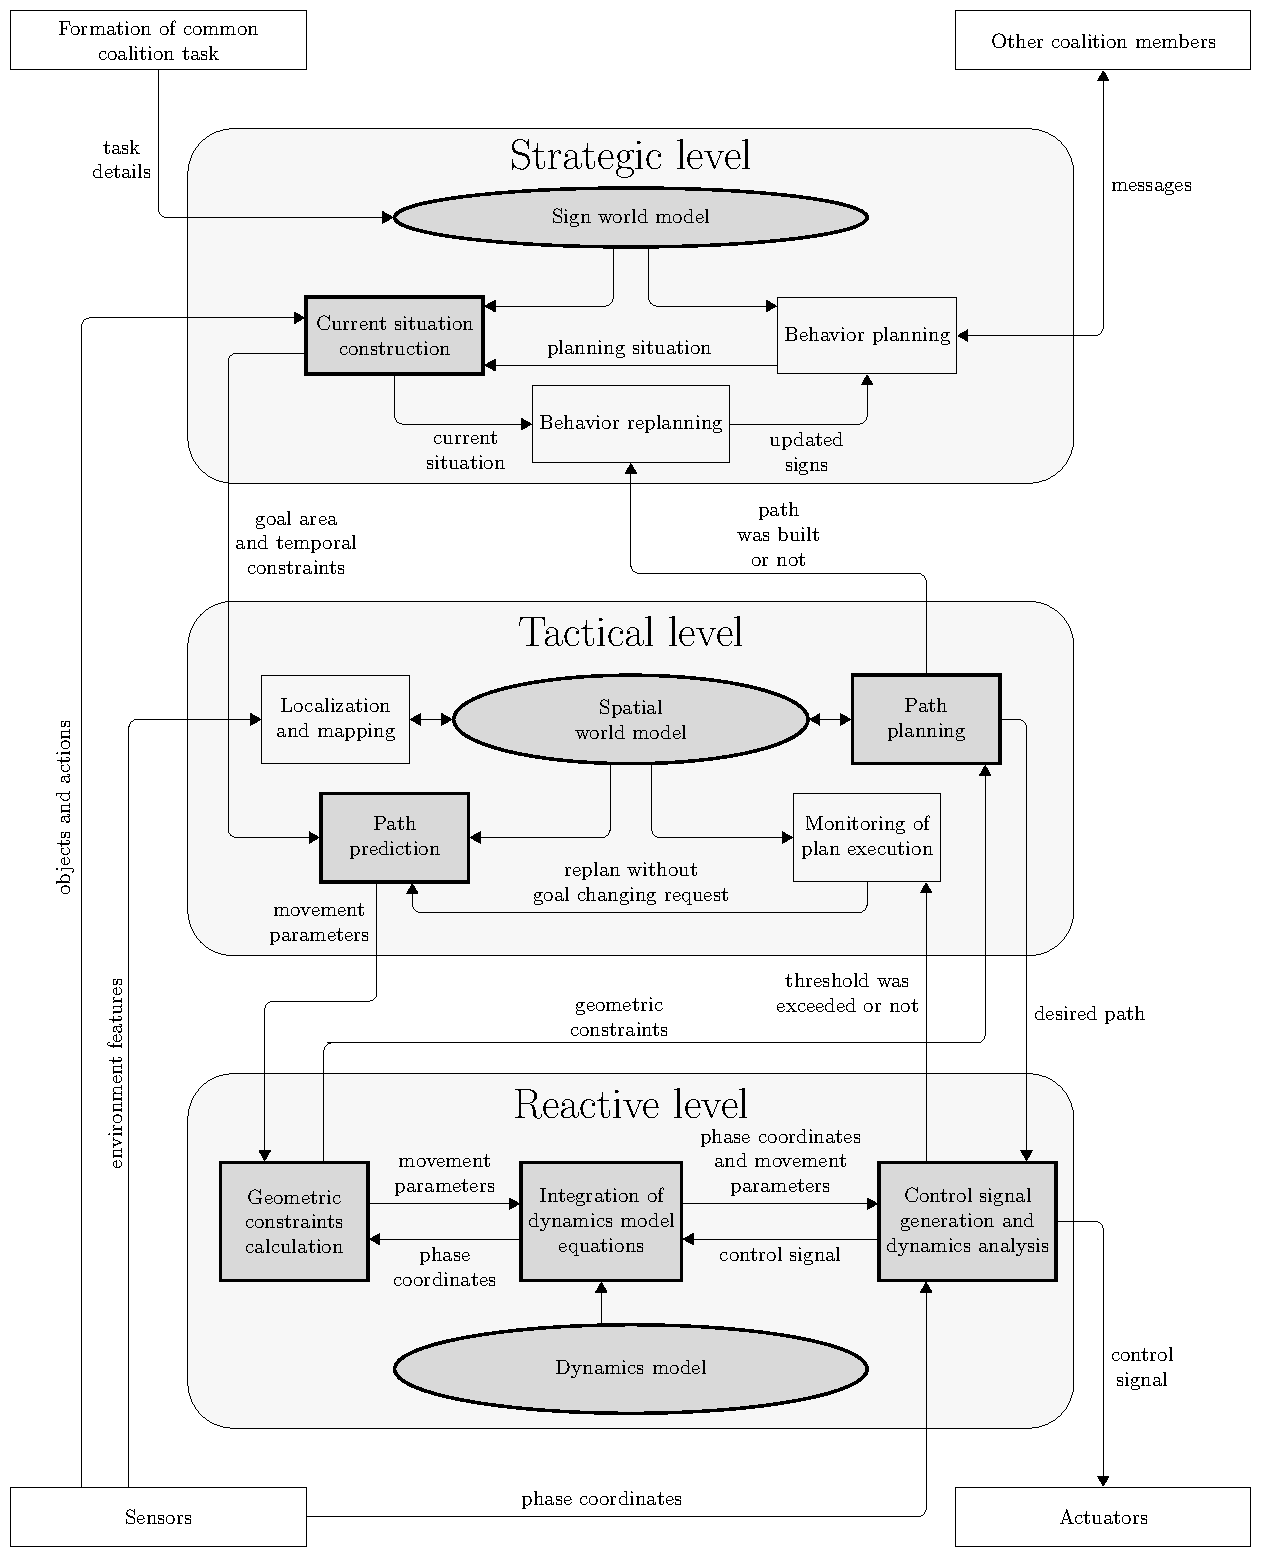
\includegraphics[width=0.9\textwidth]{agent-schemas/en/strl_arch_real_eng}
			\end{column}
		\end{columns}
		\vspace{-5pt}
		\nocite{*}
		\printbibliography[keyword={strl}, resetnumbers=true]
	\end{frame}

	\begin{frame}
		\frametitle{Symbol anchoring in robotics}
		
		\begin{columns}
			\begin{column}{0.43\textwidth}
				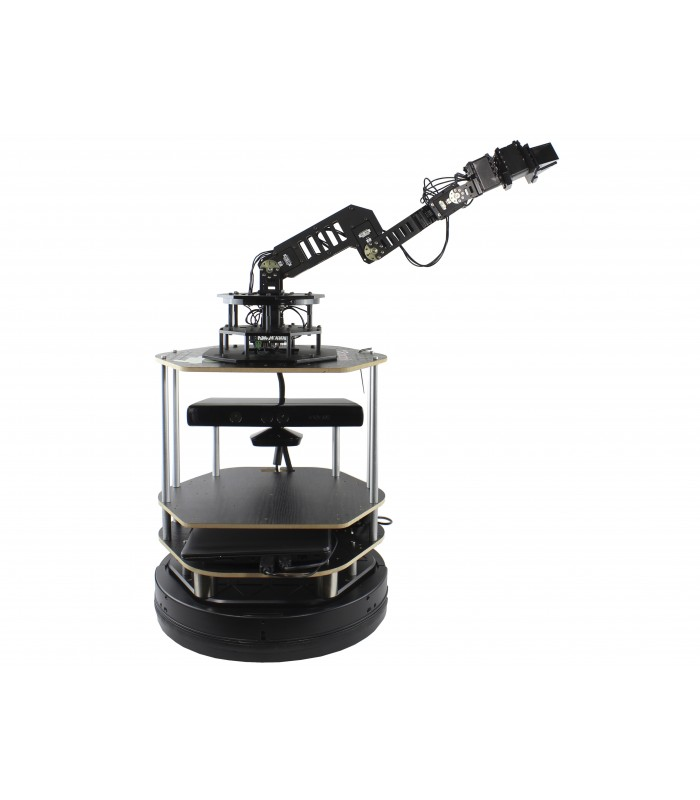
\includegraphics[width=\textwidth]{misc/agents/turtlebot-2.jpg}
				
				
			\end{column}
			\begin{column}{0.57\textwidth}
				How to form symbols, concepts and signs on the basis of sensorimotor information:
				\begin{itemize}
					\item symbol grounding problem - Harnad, 1990; Barsalou, 1999, 2008; Sun, 2013;
					\item anchoring problem - Vernon, 2014; Karpov, 2016;
					\item semiotic schemas - Roy, 2005;
					\item stream model \textbf{DyKnow} - Heintz, 2010;
					\item \textbf{conceptors} - Jaeger, 2014;
					\item \textbf{SemLinks} system - Butz, 2016, 2017.
				\end{itemize}
			\end{column}
		\end{columns}
	\end{frame}

	\begin{frame}
		\frametitle{Learning rules of relocation}
		\footnotesize
		Features of the task:
		\begin{itemize}
			\item Using reinforcement learning to form components of the sign based world model.
			\item An agent uses ``raw'' sensory information as input data.
			\item The agent's task is to form a sign based world model as a result of learning: a certain conceptual description of the environment, including discrete rules of action in it.
			\item A broader formulation is the task of joint planning in a space with role distribution and communication in a coalition.
		\end{itemize}
		\begin{center}
			\scalebox{0.35}{
				\animategraphics{12}{examples/plan/slides_colored}{}{}			
			}
		\end{center}
	\end{frame}


	\section{Problem statement}
	\subsection{Reinforcement learning}
	\begin{frame}
		\frametitle{Reinforcement learning: general statement}
		\textbf{General definitions:}
		\begin{itemize}
			\item $a_t: s_t\rightarrow s_{t+1}$ - agent's actions in the environment,
			\item $r_t$ - reward received by the agent from the environment,
			\item The agent's goal is to maximize the total reward $R=\sum\limits_{t}{{{\gamma }^{t}}}{{r}_{t}}$, $0<\gamma\le 1 $,
			\item $\pi :S\rightarrow A$ - agent's policy, taking into account previous experience and the need to study the environment: exploration and exploitation ($\epsilon$-greedy method).
		\end{itemize}
	
		\textbf{Solutions:}
		\begin{itemize}
			\item If we know $T(s_t,a_t,s_{t+1})$ and $r(s_t,a_t)$, then this is a problem based on the model and we should solve a \textit{Bellman equation}.
			\item Evaluation of value function $V(s)=\mathbf{E}[R|s,\pi]$ or action-value function $Q(s,a)=\mathbf{E}[R|s,a,\pi]$.
		\end{itemize}
	\vspace{-5pt}
	\nocite{*}
	\printbibliography[keyword={rlearn}, resetnumbers=true]
	\end{frame}
	
	\begin{frame}
		
		\frametitle{Reinforcement learning: relocation rules}
		\begin{columns}
			\begin{column}{0.7\textwidth}
				\begin{itemize}
					\item $E=(M,G)$ - environment, where $M$ - local map, $G(p_s,p_f)$ - an algorithm of reward generation,
					\item $a_t=p_t\rightarrow p_{t+1}$ - relocation actions of the agent,
					\item $s_t\in R^{(2d)^2}$ - agent's observation (sensory information).
				\end{itemize}
			\end{column}
			\begin{column}{0.3\textwidth}
				\centering
				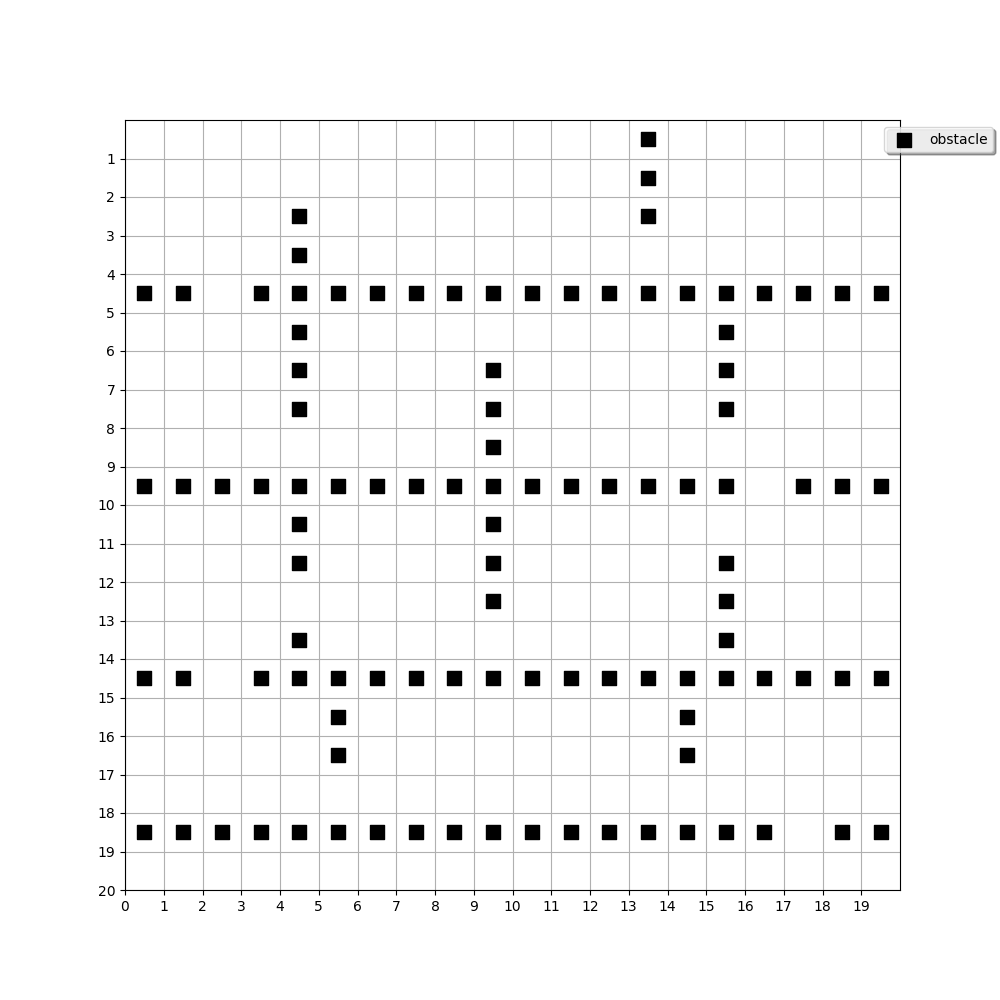
\includegraphics[width=\textwidth]{examples/path/map1}
			\end{column}
		\end{columns}
		\vspace*{10pt}
		Lets ${{Q}^{*}}({{s}_{t}},{{a}_{t}})={{\max }_{\pi }}\mathbf{E}[R|{{s}_{t}},{{a}_{t}},\pi ]$ - optimal action-value function, then taking into account the definition of $R$ \tikz[baseline] \node[coordinate] (n1) {}; we receive the Bellman equation:
		\begin{equation*}
			Q^*(s,a)=\mathbf E_{s_t\sim E}\left[
			\tikz[baseline]{
				\node[fill=blue!20,anchor=base] (t1)
				{$r_t+\gamma\max_{a_t}Q^*(s_t,a_t)$};
			}
			|s,a \right]
		\end{equation*}
		\begin{tikzpicture}[overlay]
			\path[->] (n1.south) edge [bend left, out = -50] (t1);
		\end{tikzpicture}
	\end{frame}

	\begin{frame}
		\frametitle{Reinforcement learning: approximation}
		
		To solve the Bellman equations by means the iterative methods it is used different approximations of the function ${{Q}^{*}}(s,a)$: $Q(s,a;\theta )\approx {{Q}^{*}}(s,a)$. 
		\par\medskip
		During the learning process parameters $\theta$ are adjusted as a result of minimization of the loss function $L(\theta)$:
		
		\begin{multline*}
			L_i(\theta_i)=\mathbf E_{s,a\sim\rho(\cdot)}\left[(
			\tikz[baseline]{
				\node[fill=blue!20,anchor=base] (t1)	
				{$y_i$};
			}
			-Q(s,a;\theta_i))^2\right],\\
			y_i=
			\tikz[baseline]{
				\node[fill=green!20,anchor=base] (t2)
				{$\mathbf E_{s_t\sim E}\left[r_t+\gamma\max_{a_t}Q(s_t,a_t;\theta _{i-1})|s,a \right]$};
			}
		\end{multline*}
		
		\begin{multline*}
			{{\nabla }_{{{\theta }_{i}}}}{{L}_{i}}({{\theta }_{i}})={{\mathbf{E}}_{s,a\sim \rho (\cdot );{{s}_{t}}\sim E}}\left[ \left( {{r}_{t}}+\gamma {{\max }_{{{a}_{t}}}}Q({{s}_{t}},{{a}_{t}};{{\theta }_{i-1}}) \right. \right.- \\ 
			\left. \left. -Q(s,a;{{\theta }_{i}}) \right){{\nabla }_{{{\theta }_{i}}}}Q(s,a;{{\theta }_{i}}) \right].
		\end{multline*}
			

		\begin{tikzpicture}[overlay]
			\path[<-] (t1.north) edge [bend left,in = 120] (t2);
		\end{tikzpicture}
	\end{frame}

	\begin{frame}
		\frametitle{Reinforcement learning: replays}
		\begin{itemize}
			\item An episode is a set of agent's actions and reactions of the environment to movements from the initial position to the final, or until the maximum number of actions $N_a$ is reached ,
			\item $e_t=(s_t,a_t,r_t,s_{t+1})$ - a precedent saved into a memory $D$,
			\item Learning takes place according to some random sample $e$ \tikz[baseline] \node[coordinate] (n1) {}; from the memory
		\end{itemize}
	
		\begin{equation*}
			D=\left\{ e_1, 
				\tikz[baseline]{
					\node[fill=blue!20,anchor=base] (t1)
					{$e_2$};
				}
			,\dots, 
				\tikz[baseline]{
					\node[fill=blue!20,anchor=base] (t2)
					{$e_i$};
				}
			,e_{i+1},\dots e_j,
				\tikz[baseline]{
					\node[fill=blue!20,anchor=base] (t3) 
					{$e_{j+1}$};
				}
			,\dots \right\}
		\end{equation*}
		\begin{tikzpicture}[overlay]
			\path[->] (t1) edge [bend left, out = 50, in=-150] ([xshift=-10pt,yshift=-2pt]n1);
			\path[->] (t2) edge [bend left, out = 40, in=-130] ([xshift=-6pt,yshift=-2pt]n1);
			\path[->] (t3) edge [bend left, out = 30, in=-90] ([xshift=-2pt,yshift=-2pt]n1);
		\end{tikzpicture}
		\begin{itemize}
			\item One action can be used several times $\rightarrow$ expand the sample, eliminate the correlation of neighboring states.
		\end{itemize}
	\end{frame}
	
	\begin{frame}
		\frametitle{Reward generation}
		
		The following algorithm was used to calculate the reward function:
		\begin{equation*}
			G(s,g,t)=\begin{cases}
				\alpha_{opt}r_t^{opt}+\alpha_{rat}r_t^{rat}+\alpha_{euq}r_t^{euq}, & p_t\leftarrow 0,\\
				r^{obs}, & p_t\leftarrow 1,\\
				r^{tar}, & p_t=g,
			\end{cases}
		\end{equation*}
		where 
		\begin{itemize}
			\item $\sum\alpha_i=1$ - normalization,
			\item $r_t^{opt}=l_t-l_{t-1}$ - changing optimal distance,
			\item $r_t^{rat}=e^{-l_t/l_0}$ - penalty for deviation from a goal,
			\item $r_t^{euq}=|p_t-g|-|p_{t-1}-g|$ - regularizer for straightening a path.
		\end{itemize}
	\end{frame}

	\subsection{Architectures of regressors}
	\begin{frame}
		\frametitle{Heterarchical causal network}
		Biologically inspired learning model (formation of the sign component):
		\begin{itemize}
			\item scanning receptive field - pattern formation,
			\item spatial pooler (clasterization by online K-means),
			\item temporal pooler (agglomerative clasterization $\rightarrow$ Markovian chains).
		\end{itemize}
		\centering
		\vspace*{-3pt}
		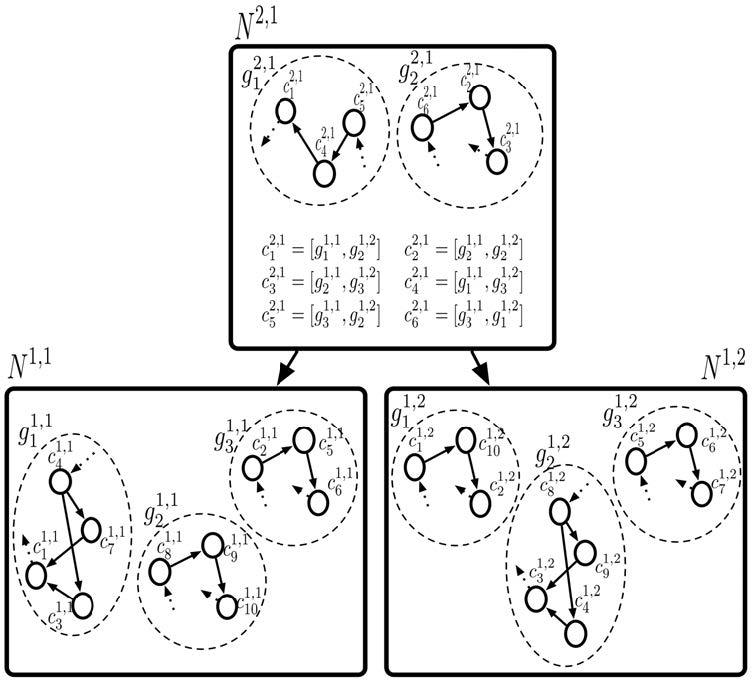
\includegraphics[width=0.39\textwidth]{misc/mpf/hawkins_htm.jpg}
	\end{frame}

	\begin{frame}
		\frametitle{Neuronal architectures}
		In the work we conducted experiments with various neural networks:
		\begin{enumerate}
			\item $Ag_1$ - a <<shallow>> fully-connected neural network,
			\item $Ag_2$ - a convolution network of medium depth with a fully connected output layer,
			\item $Ag_3$ - a deep network with Inception blocks.
		\end{enumerate}
		\centering
		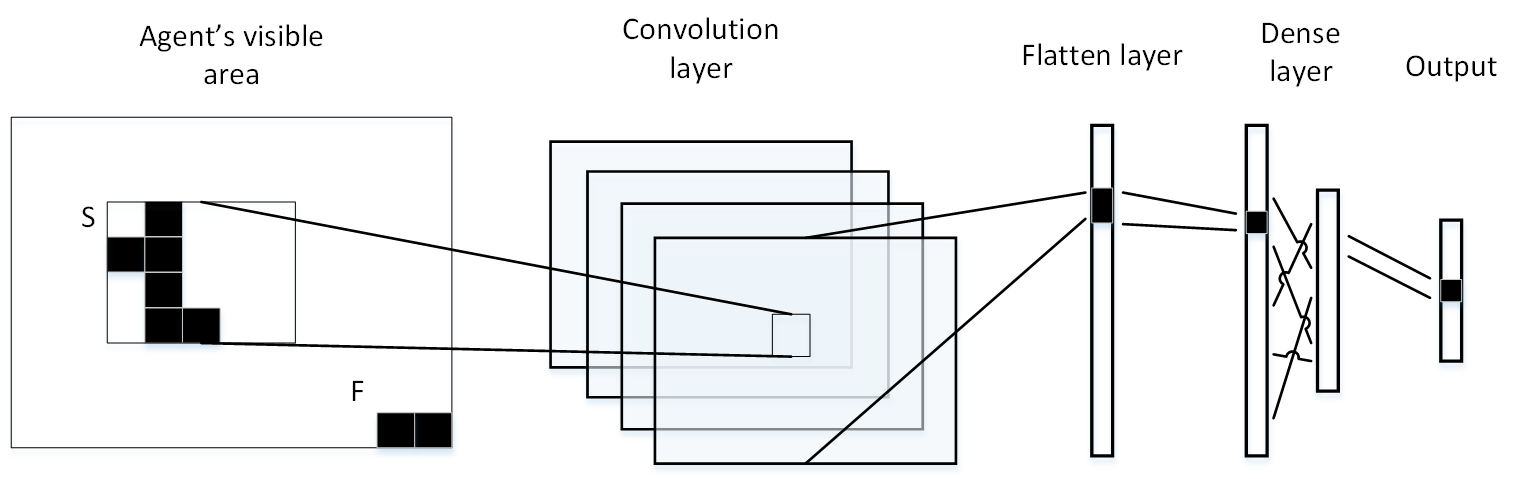
\includegraphics[width=0.8\textwidth]{examples/path/neural_arch.png}
	\end{frame}

	\section{Experiments}
	\begin{frame}
		\frametitle{Maps, paths and parameters}
		The most successful set of parameters:
		\begin{itemize}
			\item $N_{ep}\sim 3000$ - number of episodes, $N_a=100$ - maximum number of steps, $d=20$ - observation radius of the agent,
			\item $\alpha_{opt}=0.8,\alpha_{rat}=0.1$ - reward coefficients,
			\item $r^{obs}=-4,r^{tar}=10$ - reward parameters,
			\item $N_e=10$ - size of the memory $D$,
			\item $\gamma=4$ - discounting multiplier for reward function.
		\end{itemize}
		\centering
		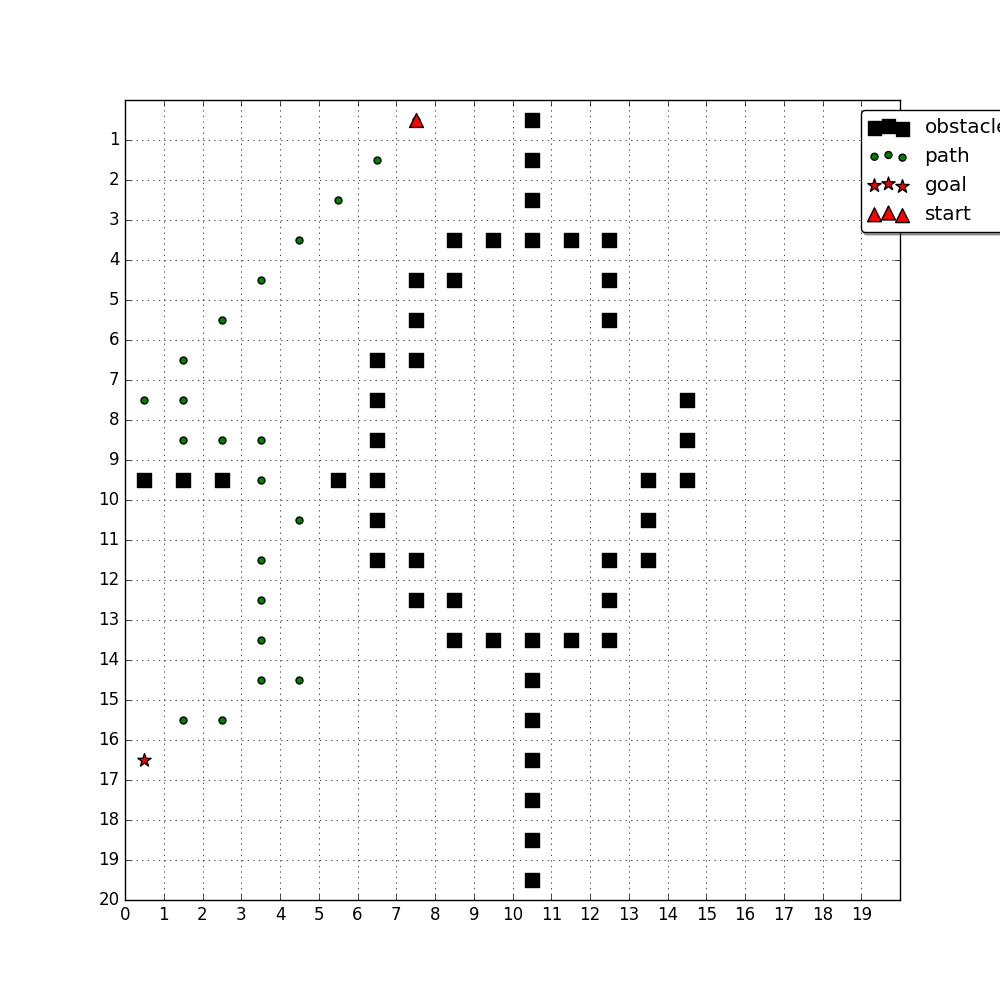
\includegraphics[width=0.35\textwidth]{examples/path/path_example.png}
		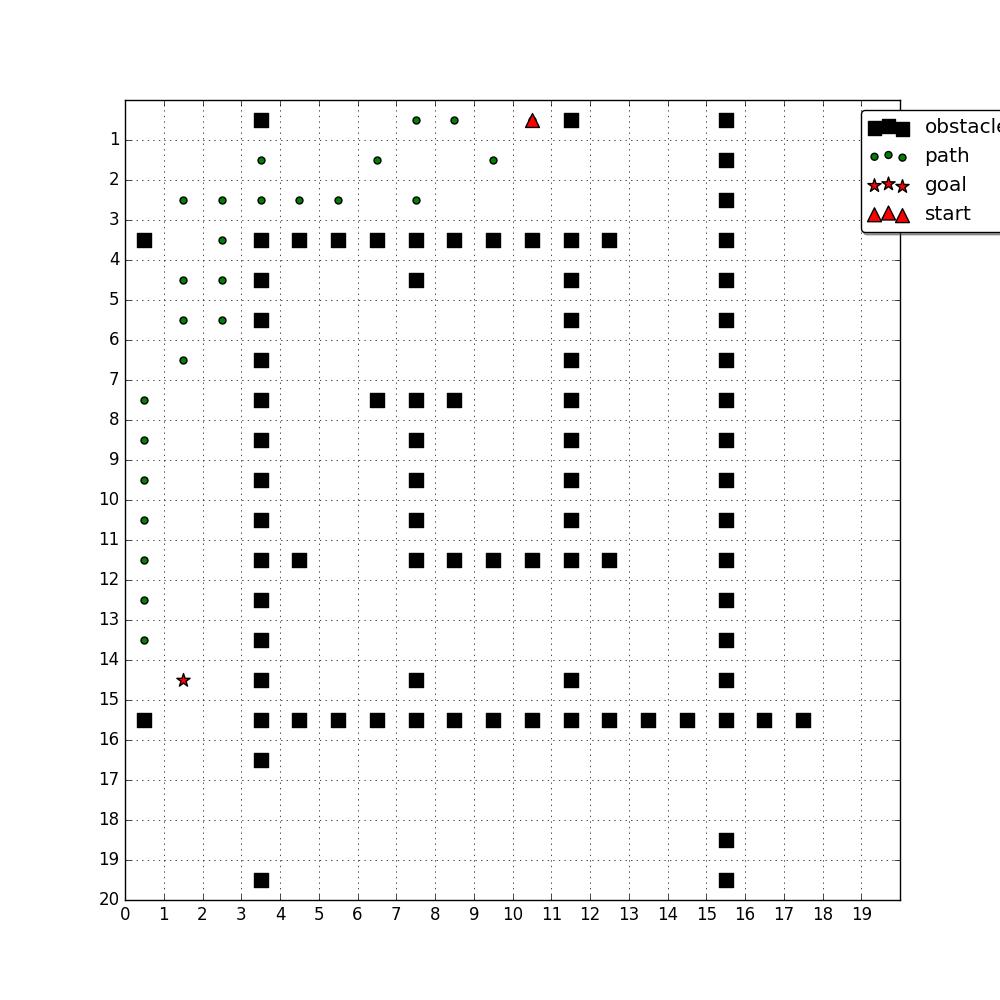
\includegraphics[width=0.35\textwidth]{examples/path/path_example_2.png}
	\end{frame}

	\begin{frame}
		\frametitle{Convergence of the learning process}
		\begin{columns}
			\begin{column}{0.65\textwidth}
				\centering
				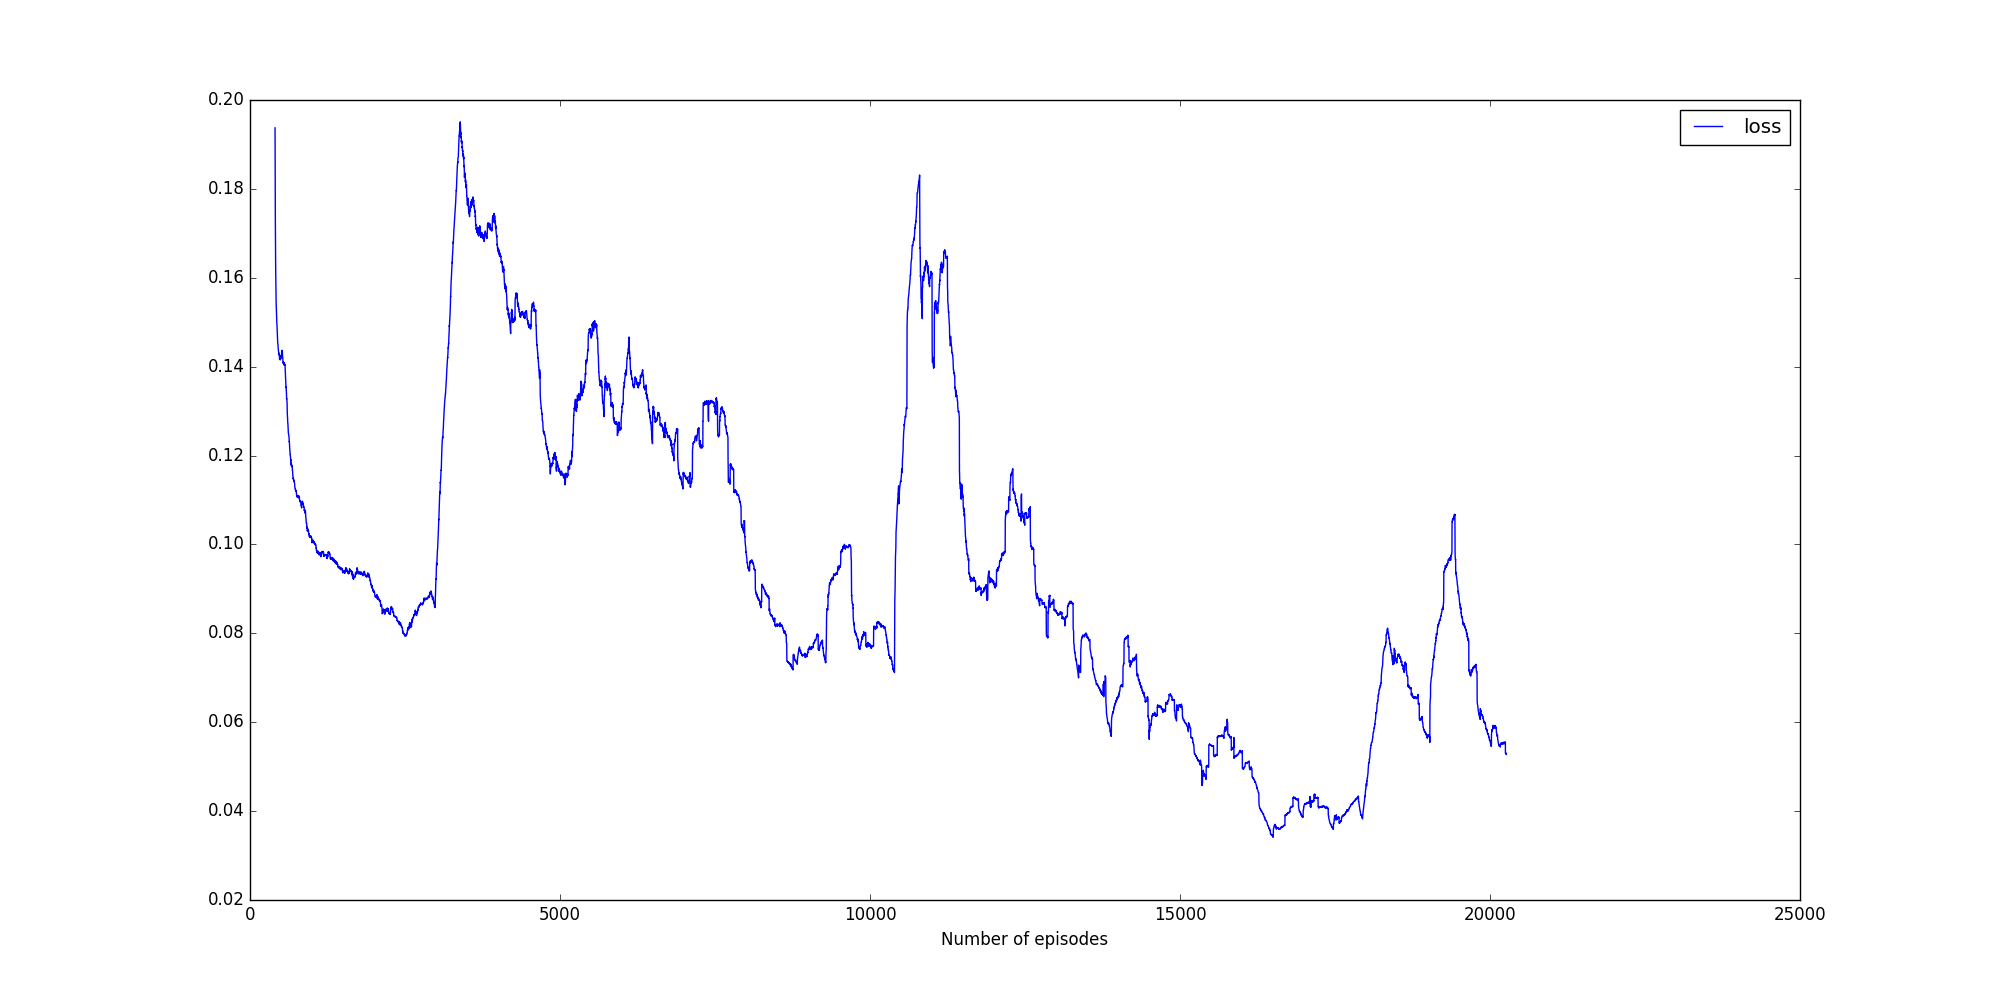
\includegraphics[width=\textwidth]{examples/path/batch_full_smoothed.png}
				\vspace*{-10pt}
				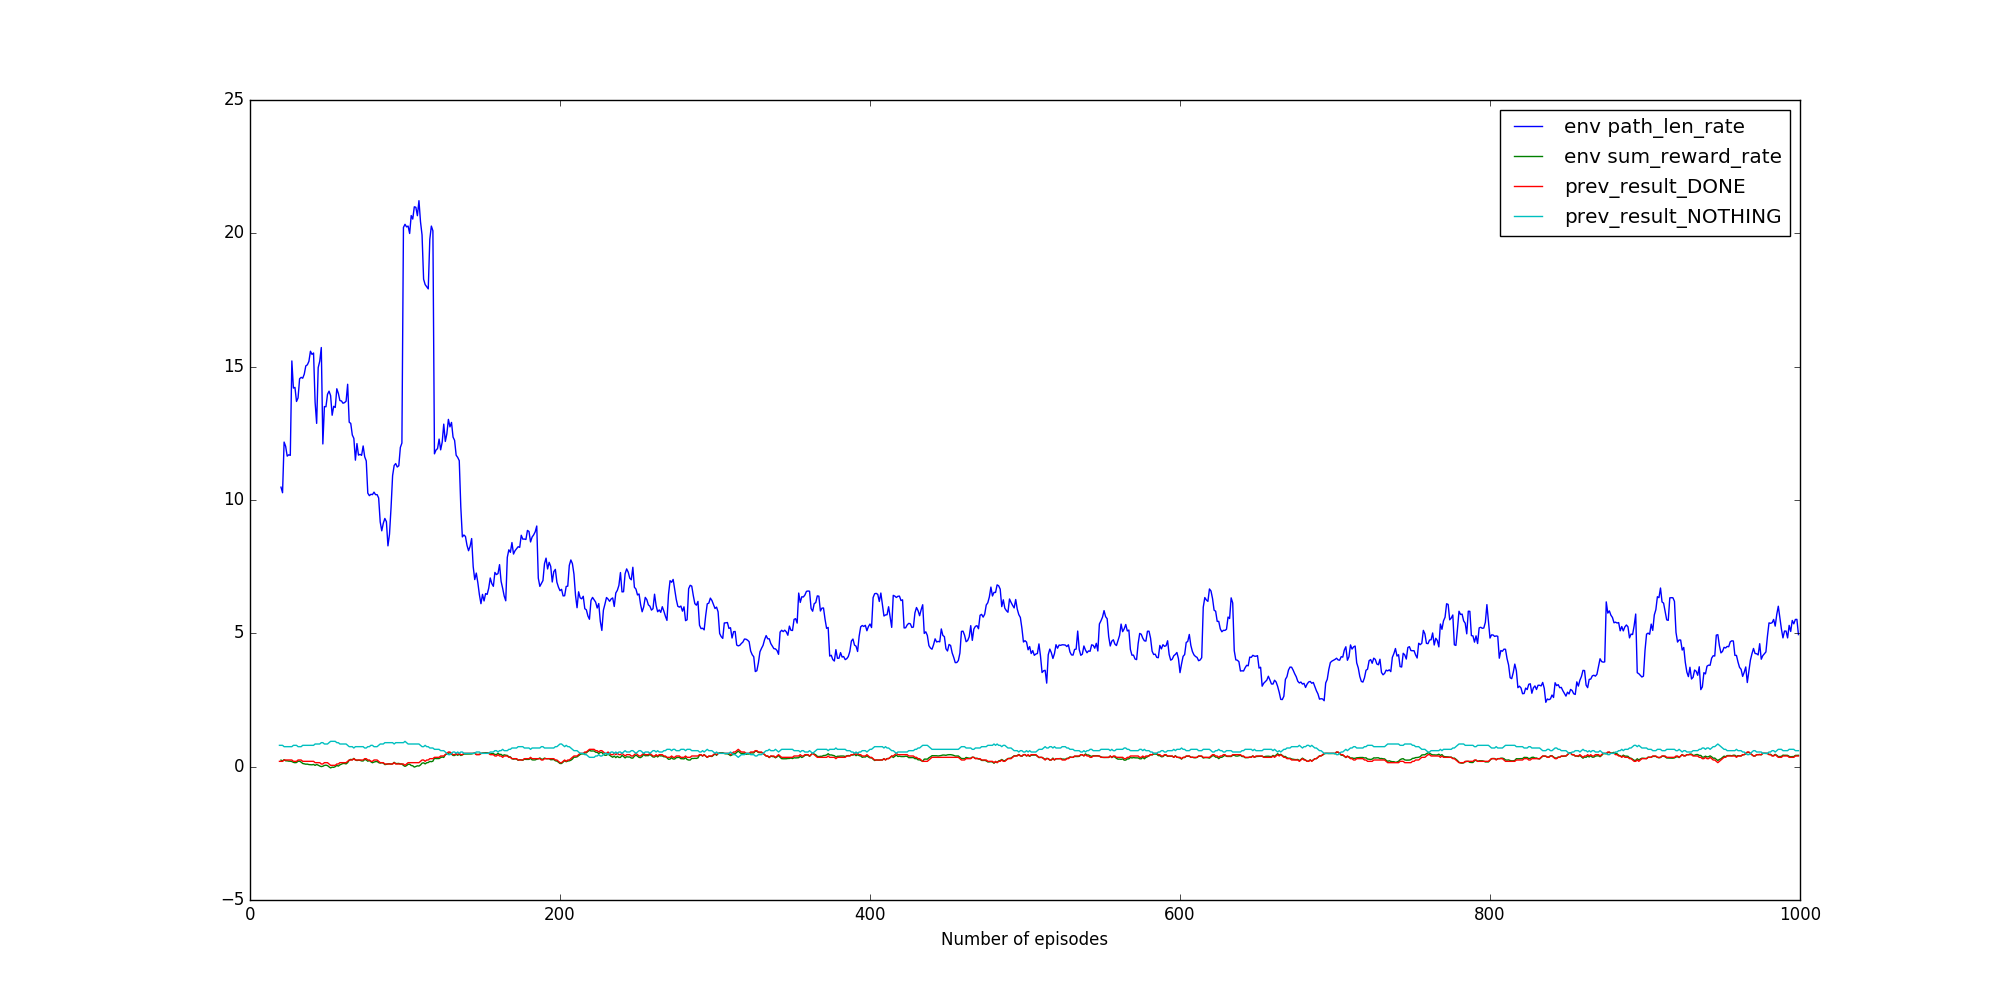
\includegraphics[width=\textwidth]{examples/path/run_episodes_smoothed.png}
			\end{column}
			\begin{column}{0.35\textwidth}
				We used two quality metrics:
				\begin{itemize}
					\item $M_p$ - the ratio of the path length found by the agent to the optimal,
					\item $M_r$ - the ratio of total reward to its maximum value.
				\end{itemize}
			\end{column}
		\end{columns}
		
		
	\end{frame}

	\begin{frame}
		\centering
		\Huge
		Thank you for your attention!
		\normalsize
		\par\bigskip
		\par\bigskip
		\par\bigskip
		pan@isa.ru
	\end{frame}			
\end{document}
	
	
